%%%%%%%%%%%%%%%%%%%%%%%%%%%%%%%%%%%%%%%

\chapter{  État de l'art \label{Chap:SOA}}

Dans le Chapitre \ref{Chap:SOA} nous présentons les différentes caractéristiques de notre problème, étudions la classe de problème auquel il appartient et par la même occasion nous définissons sa complexité. Dans le même temps nous étudions les applications actuelles liées aux problèmes de la classe pour déterminer les limites de ces problèmes par rapport aux données réelles. Notre problème appartient à la classe des problèmes d'ordonnancement et de routage d'employés (\textit{Workforce Scheduling and Routing Problem} en anglais, noté $\wsrp$).



%%%%%%%%%%%%%%%%%%%%%%%%%%%%%%%%%%%%%%%
%%%%%%%%%%%%%%%%%%%%%%%%%%%%%%%%%%%%%%%

%\section{Applications actuelles}
\label{sec:SOA_AppAct}
Les problèmes de la classe \wsrp ~sont très présents dans la littérature, il existe plusieurs domaines d'applications dans le milieu industriel (voir \cite{Castillo2016} qui propose une liste d'applications), chacun de ces domaines apporte ses contraintes et ses objectifs spécifiques. 

On propose d'étudier tout de même les problèmes qui ne présentent que la composante de routage (e.g. Vehicule Routing Problem) et ceux qui ne présentent que la composante d'ordonnancement (e.g. Technician and Task Scheduling Problem, \ttsp, ou Nurse Rostering Problem) car on pourrait étendre leurs mécanismes de résolution à notre problème. La plupart de ces problèmes ne diffèrent que de quelques contraintes : par exemple, \ttsp ~autorise le travail en équipe, alors que le problème de planning d'infirmière ne l'autorise pas. 

Comme pour tous les problèmes d'optimisation, plusieurs méthodes de résolution s'opposent : les méthodes exactes, les méthodes approchées avec garanties de performances, les méthodes \mbox{(méta-)}\\heuristiques ou les méthodes hybrides qui mélangent les méthodes de résolutions ci-dessus. 
Le choix des méthodes de résolution est fortement lié aux critères de résolution du problème, par exemple si l'on peut se permettre de résoudre le problème à l'optimal dans un temps raisonnable, on va favoriser les méthodes exactes; sinon on va s'orienter vers les méthodes approchées ou hybrides.
Les méthodes approchées visent à obtenir une "bonne" solution rapidement avec une garantie sur l'écart entre la valeur de la fonction objectif de la solution trouvée avec l'algorithme approché par rapport à la valeur de la fonction objectif de la solution optimale.
\begin{mydef}
\label{def:exact}
Une méthode exacte parcourt l'arbre de recherche du problème afin de trouver la meilleure solution avec une garantie d'optimalité.
\end{mydef}
\begin{mydef}
\label{def:greedy}
Un algorithme glouton (greedy algorithm) est un algorithme qui étape après étape améliore la solution actuelle jusqu'à un extremum local (parfois global). 
\end{mydef}
\begin{mydef}
\label{def:metaheuristic}
Une méta-heuristique est une méthode permettant de trouver un extremum local pour un problème d'optimisation. Le fonctionnement général d'une méta-heuristique est de parcourir un "voisinage" d'une solution courante en cherchant a optimiser une fonction objectif. Il existe un grand nombre de méta-heuristiques allant de la simple recherche locale vers des algorithmes génétiques aux comportements plus complexes.
\end{mydef}

Dans un premier temps, nous allons présenter les différents problèmes d'ordonnancement proches des problèmes de \wsrp ~que nous avons pu rencontrer dans la littérature, ainsi que leur complexité, puis nous ferons de même avec les problèmes de routage.




%%%%%%%%%%%%%%%%%%%%%%%%%%%%%%%%%%%
%%%%%%%%%%%%%%%%%%%%%%%%%%%%%%%%%%
\section{Ordonnancement \label{sec:SOA_APPAct_Ordo}}

Dans cette section nous nous intéressons aux problèmes d'ordonnancement proche de notre problème.
Définissons tout d'abord un problème d'ordonnancement :
\begin{mydef}
Un problème d'ordonnancement consiste à organiser des tâches dans le temps en respectant des contraintes temporelles et des contraintes de ressources.
\end{mydef} 
La composante d'ordonnancement est très présente dans les problèmes de \wsrp.
Les problèmes d'ordonnancement sont classifiés selon trois champs $\alpha~|~\beta~|~\gamma$.
Le champ $\alpha$ correspond aux contraintes sur les machines (nombre de machines, etc).
Le champ $\beta$ correspond aux contraintes entre les machines (précédence, préemption, etc) et aux contraintes de ressources.
Le champ $\gamma$ correspond à la fonction objectif que l'on veut optimiser (minimiser la complétion totale du planning, minimiser le retard des tâches, etc). 
Tous les champs appartiennent à $\alpha~|~\beta~|~\gamma$ sont détaillés dans le livre \cite{blazewicz2007handbook}.
Par exemple le problème $1~|~\textit{prec}~|~C_{max}$ correspond à l'ordonnancement de tâches sur une machine, les tâches ont des contraintes de précédences et on souhaite minimiser la complétion totale de l'ordonnancement.

Les problèmes d'ordonnancement sont regroupés dans la classe \ssp, cette classe a été définie par Graham et al. \cite{Graham1979}, ils présentent la complexité et les approximations de certains problèmes ; Lawler et al. \cite{Lawler1993} proposent des algorithmes pour résoudre ces problèmes.
\begin{mydef}
La classe \ssp ~est la classe des problèmes définis par l'allocation optimale de ressources rares pour des activités dans le temps.
La classe \ssp ~représente tous les problèmes d'ordonnancement classiques (ordonnancement sur une machine, ordonnancement de machines parallèles, OpenShop, FlowShop, JobShop, $\ldots$).
\end{mydef}

Les problèmes d'ordonnancement qui ressemblent le plus aux problèmes de la classe \wsrp ~sont les problèmes de la classe \mpsp (problème d'ordonnancement de projet à compétences multiples ou Multi-Skill Project Scheduling Problem en anglais). Les problèmes de la classe \mpsp ~consistent à trouver un ordonnancement réalisable des tâches en respectant les contraintes de précédence et de ressources : un employé/une machine peut effectuer une tâche que s'il/si elle possède les compétences et ressources requises.

Firat \cite{Firat2012} montre que le problème MPSP est $\np$-difficile, Blazewicz \cite{Blazewicz1983} montre que le problème d'ordonnancement de projet avec contrainte de ressources (resources constrainted project scheduling problem en anglais, noté RCPSP) est $\np$-difficile au sens fort. L’œuvre de synthèse  \cite{Graham1979} définit différents problèmes d'ordonnancement et leur approximation.

On retrouve des problèmes proches de ceux des \wsrp ~dans la littérature comme le problème de planning d'infirmières dans \cite{Trilling2007} ou dans \cite{Burke2010}.
L’œuvre de synthèse de Burke \cite{burke2004state} pose un état de l'art sur les problèmes de planning d'infirmières.
Le problème de planning d'infirmières est un problème qui possède beaucoup de contraintes souvent séparées en contraintes "molles" (soft constraints en anglais) qui peuvent être violées mais a un certain coût et contraintes "dures" (hard constraints en anglais) qui ne peuvent pas être violées. 
Les contraintes molles sont souvent les contraintes liées aux préférences des infirmières et les contraintes dures représentent les contraintes sur le temps de travail ou autres particularités qui sont assez réglementées.

La Figure~\ref{nurseRostering} montre un planning d'infirmières sur cinq jours avec deux sortes de "shifts" (early et late) avec des infirmières à temps plein et des infirmières à temps partiel et une demande de personnel pour chaque shift pour chaque jour.


\begin{figure}[H]
\centering
\includegraphics[scale=0.3]{nurseRostering.png}
\caption{Exemple de planning d'infirmières\label{nurseRostering}}
\end{figure}

Un autre problème d'ordonnancement proche des problèmes des \wsrp ~est le problème d'ordonnancement de techniciens et de tâches (\ttsp). \ttsp ~a été le sujet du challenge de 2007 de la ROADEF \cite{Cordeau2010,Pokutta2009,Hurkens2009}.
C'est un problème très présent dans le domaine de la télécommunication.
Dutot \cite{dutot2006technicians} définit le problème \ttsp. 
Hurkens et al.\cite{Hurkens2009} sont les vainqueurs de la compétition en utilisant la programmation linéaire mixte (Mixed Integer Programming) : ils utilisent une méthode de résolution en deux phases. 
La première pour obtenir de bonnes bornes inférieures et déterminer quelles tâches doivent être sous-traitées. 
La deuxième phase affecte les meilleurs couples tâche/technicien  en utilisant un algorithme de couplage.
Cordeau et al.\cite{Cordeau2010} finissent deuxième en utilisant des méthodes hybrides, programmation linéaire et heuristiques : recherche de voisinage large adaptatif \ref{def:ALNS}(Adaptative Large Neighborhood Search en anglais) et heuristique de construction.
Pokutta et al.\cite{Pokutta2009} terminent cinquième en se basant sur des méthodes heuristiques et de la recherche locale. 
Firat et al.\cite{Firat2012} améliorent la méthode de résolution de Hurkens et al.\cite{Hurkens2009} en trouvant de meilleures bornes inférieures dans la première phase. Ils obtiennent de meilleurs résultats. 

\begin{mydef}
\label{def:ALNS}
La recherche de voisinage large adaptatif (Adaptative Large Neighborhood Search en anglais) introduite par \cite{Ropke2005}, est une heuristique qui étend la méta-heuristique Large Neighborhood Search proposée par \cite{shaw1998using} et est très proche de l'heuristique de destruction et de réparation de \cite{schrimpf2000record}. Le comportement de l'heuristique est le suivant : en partant d'une solution initiale, on dégrade/détruit une partie de la solution pour ensuite la reconstruire de manière optimale (localement). En enchaînant successivement ces deux étapes, on espère obtenir une solution de meilleure qualité. Cette méthode a d'abord eu de nombreux succès pour les problèmes de routage, puis s'est étendue vers de nombreux autres problèmes comme les problèmes d'ordonnancement.
\end{mydef}


%%%%%%%%%%%%%%%%%%%%%%%%%%%%%%%%%%%
%%%%%%%%%%%%%%%%%%%%%%%%%%%%%%%%%%

\section{Routing \label{sec:SOA_APPAct_Routing}}
Dans cette section, nous détaillons les problèmes de routage proches de notre problème.
Généralement les problèmes de routage sont définis sur des graphes.
Un problème de routage peut être défini de la manière suivante \cite{lenstra1981complexity} :
\begin{mydef}
Soit $G=(V,E,A)$ un graphe "mixte" (mixed graph en anglais) fortement connexe, avec V représentant l'ensemble des sommets, E les arêtes et A les arcs\footnote{\label{refnote} arc est orienté alors qu'une arête ne l'est pas}. Étant donné $V'\subseteq V$, $E'\subseteq E$ et $A'\subseteq A$ et des coûts positifs sur les arêtes et arcs, trouver une tournée de coût minimum passant par $V',~E'$ et $A'$. \label{def:sVRP}
\end{mydef}

Cette définition caractérise les problèmes de routage à un seul véhicule comme par exemple le problème du voyageur de commerce (travelling salesman problem en anglais, noté TSP (c.f. Problème~\ref{pb:TSP}), en utilisant la définition précédente on peut exprimer le TSP en utilisant $V' = V,~E'=\emptyset$ et $A' =\emptyset$ : on doit passer par tous les sommets sans restriction sur les arêtes ou arcs utilisées.

\begin{problem}{Traveling Salesman Problem}{TSP}
\label{pb:TSP}
\probdef
{Un graphe complet pondéré $G=(V,E,\omega)$ non orienté et $k$ un entier.}
{Existe-t-il un cycle hamiltonien\footnotemark de coût $\leq k$ ? }
{}{}{def:TSP}
\end{problem}
\footnotetext{Un cycle Hamiltonien est un cycle qui passe par tous les sommets d'un graphe une et une seule fois.}

Le problème Traveling Salesman Problem (Problème~\ref{pb:TSP}) a été montré $\np$-complet par Papadimitrou \cite{papadimitriou1977euclidean} même pour les instances qui peuvent être représentées dans un plan euclidien.

On peut étendre la définition~\ref{def:sVRP} pour caractériser les problèmes de routage avec plusieurs véhicules : 

\begin{mydef}
Soit $G=(V,E,A)$ un graphe "mixte" (mixed graph en anglais) fortement connexe, avec V représentant l'ensemble des sommets, E les arêtes et A les arcs\footref{refnote} et $m$ un entier. Étant donné $V'\subseteq V$, $E'\subseteq E$ et $A'\subseteq A$ et des coûts positifs sur les arêtes et arcs, trouver $m$ tournées disjointes de coût minimum passant par $V',~E'$ et $A'$. \label{def:mVRP}
\end{mydef}

Cette définition nous permet d'exprimer le "multiple Travelling Salesman Problem" (m-TSP). En ajoutant des contraintes de capacité sur les véhicules et des coûts sur les sommets, on obtient le problème suivant  :
\begin{problem}{multiple Capacited Vehicule Routing Problem}{mCVRP}
\label{pb:VRP}
\probdef{Un graphe pondéré $G=(V,E,\omega)$ non orienté, $|V|=n+1$ le sommet $0$ représente le dépôt et les $n$ représente les clients, pour chaque client il y a une demande $d_i$, $m$ véhicules de capacité $Q$.}{Trouver au plus $m$ cycles sommet-disjoints de coût Min couvrant $V\backslash\{0\}$ commençant et terminant en 0, respectant les capacités des véhicules et les demandes des clients.}{}{}{def:VRP}
\end{problem}

Si les véhicules ont les mêmes caractéristiques on dit que les véhicules sont homogènes (homogeneous fleet en anglais).

Ajouter des contraintes temporelles supplémentaires ne peut que rendre le problème plus difficile \cite{Tsitsiklis1992}, les variantes du TSP avec des fenêtres temporelles (Traveling Salesman Problem with Time Windows) sont donc $\np$-difficiles.
Les fenêtres temporelles peuvent être uniquement sur les clients (sommets) ou alors  à la fois sur les véhicules et les clients (horaires de travail pour les personnes conduisant les véhicules). Il peut aussi y avoir plusieurs intervalles pour chaque fenêtre temporelle \cite{beheshti2015vehicle}. 
Desrosiers et al. \cite{Desrosiers1995} montrent que trouver une solution réalisable, pour le VRPTW avec le nombre de véhicule utilisé fixé, est $\np$-difficile.
Les algorithmes utilisés pour résoudre le problème supposent que le nombre de véhicules n'est pas borné.
Ce qui implique de déterminer le nombre de véhicules a utiliser et l'ensemble des tournées optimales pour ces véhicules.
Comme le Vehicule Routing Problem with  Time Windows (VRPTW)  est une variante du problème TSPTW, VRPTW est donc $\np$-difficile.
Tous les résultats de $\np$-complétude sont montrés au sens fort \cite{garey1978strong}, ce qui implique qu'il n'existe pas de schéma d'approximation polynomial. Empiriquement, il s'avère que les problèmes $\np$-complets au sens fort sont plus difficiles à résoudre.
Tsitsiklis et al. \cite{Tsitsiklis1992} montrent la complexité des différents problèmes de tournées de véhicules avec fenêtres temporelles.

Pour les méthodes de résolution, dans la littérature on retrouve pour les problèmes de tournées de véhicules les méthodes heuristiques LNS et ALNS ou les méthodes exactes avec la génération de colonnes et le branch and price (utilisant la programmation dynamique \cite{feillet2010,hernandez2014new}).
Solomon et al.\cite{solomon1987} ont défini des jeux d'instances qui sont devenus la référence pour comparer ses résultats.
Ces instances sont composées de 25 à 100 clients (25 à 100 sommets), il faut minimiser les déplacements et le nombre de véhicules utilisés.
Actuellement les meilleures solutions trouvées sont obtenues grâce à des (méta-)heuristiques comme l'ALNS \cite{Ropke2005} ou en utilisant la programmation par contraintes et la recherche locale \cite{shaw1998using}.


%%%%%%%%%%%%%%%%%%%%%%%%%%%%%%%%%%%%%%%
%%%%%%%%%%%%%%%%%%%%%%%%%%%%%%%%%%%%%%%

\section{Workforce Scheduling and Routing Problem (\wsrp) \label{sec:SOA_WSRP}}
Dans la section suivante, nous définissons plus formellement la classe de problème Workforce Scheduling and Routing Problem en se basant sur l'étude menée par Castillo et al. \cite{Castillo2016}. \wsrp ~représente les problèmes qui mobilisent de la main-d’œuvre pour effectuer des tâches, dans des sites/établissements, chez des clients. 
Pour ce faire, les employés doivent se déplacer en utilisant différents moyens de transport (vélo, voiture, transport en commun, $\ldots$). Les employés commencent/terminent leur journée dans un dépôt ou de leur maison respective. Les employés ont des horaires de travail journaliers et les clients ont aussi des horaires d'ouverture.

La durée des tâches n'est pas négligeable par rapport à la durée des transport, et peut dépendre de l'employé.
Les tâches ont des compétences requises qui permettent de filtrer les employés qui peuvent les réaliser.
Une tâche peut être exécutée par un ou plusieurs employés, dans ce cas tous les employés doivent être présents avant de débuter la tâche.
Il peut y avoir des dépendances temporelles entre les tâches, elles sont définies par Castillo et al. et Rasmussen et al. \cite{Castillo2015,Rasmussen2010}, certaines tâches sont donc prioritaires par rapport aux autres. 
Certaines tâches peuvent être sous-traitées.
De plus, le planning des employés peut varier, il peut être journalier, hebdomadaire, etc.

En général les instances de la classe \wsrp sont beaucoup trop grandes pour être traitées dans leur globalité, on les découpe en zones géographiques plus petites, d'une part pour éviter qu'un employé doive travailler loin de chez lui mais aussi pour réduire la taille de l'instance pour pouvoir la résoudre plus facilement/rapidement.

\begin{comment}
\begin{itemize}
\item Fenêtre temporelle (Time windows en anglais) : le temps disponible pour que la tâche puisse être effectuer par un employé.

\item Moyen de transport (Transportation modality) : le moyen de transport des employés (voiture, transport en commun, $\ldots$). On peut donc supposer que les temps de transport peuvent varier d'un employé a l'autre.

\item Point de départ et d'arrivé (Start and end point) : le point de départ des employés peut varier selon si ceux-ci peuvent commencer de leur maison ou s'ils doivent commencer depuis un local de l'entreprise. Pour le point d'arrivé soit les employés rentrent directement chez eux, à leur maison, soit les employés doivent d'abord passer par un local de l'entreprise.

\item Compétences/Qualifications (Skills/Qualification) : soit les employés ont le même niveau de compétence dans ce cas tout le monde peut effectuer toutes les tâches. Soit les employés ont des compétences différentes et donc les compétences agissent comme un filtre pour savoir qui peut ou ne peut pas effectuer une tâche.

\item Durée des tâches (Service Time) : la durée d'une tâche peut varier d'un employé à l'autre. Si la durée des tâches est longue (un employé ne peut effectuer qu'une tâche par jour) le problème correspond donc en un problème d'allocation de tâches.

\item Dépendances de tâches (Connected activities) : les tâches peuvent avoir des dépendances temporelles entre elles. Ces dépendances sont explicités dans \cite{Rasmussen2010}, mais comme dans la plupart des problèmes de d'ordonnancement on peut voir ces dépendances comme des contraintes de précédences de tâches.

\item Travail en équipe (Teaming) : lorsque les équipes ne changent pas on peut les considérer comme de simples employés. Si les équipes changent il faut constamment réorganiser les équipes pour qu'elles correspondent le mieux aux tâches. 

\item Découpage en zone (Clusterization) : lorsque les instances du problème sont beaucoup trop grandes on peut les découper en zones (cluster) pour réduire la taille du problème.

\item Sous-traitance (Out-sourcing) : la sous-traitance n'est pas défini comme critère dans \cite{Castillo2016} mais elle est assez récurrente dans la littérature des \wsrp. On peut accepter de faire certaines tâches grâce à la sous-traitance mais cela à un coût.
\end{itemize}


\rod{améliorer l'écriture de cette partie. Faire une ou plusieurs figures synthétiques}
\gab{C'est qu'un premier jet}
\end{comment}





\begin{table}[H]

\centering
\begin{tabular}{|c|c|}
\hline
Employé & Tâche\\
\hline
Moyen de transport  & Durée d'exécution \\
Position de départ & Position\\
 Position d'arrivé & Dépendance temporelle\\
 Équipe& Horaire d'ouverture\\
Horaire de travail  & Compétences requises\\
Compétences  & Priorité\\
 ~&Sous-traitance\\
\hline

\end{tabular}
\caption{\label{CharEmploy}Caractéristiques des employés et des tâches}
\end{table}

Par exemple un problème de la classe pourrait être : un ensemble d'employés qui doit effectuer un ensemble de tâches chez des clients. Les employés peuvent se déplacer en voiture, vélo ou en transport en commun pour effectuer les tâches. Les employés sont autorisés à commencer leur journée de chez eux mais doivent terminer dans un local technique de l'entreprise (pour se réapprovisionner). Le travail en équipe n'est pas autorisé. Les employés ont des compétences spécifiques dans certains domaines. Les horaires de travail ne sont pas fixés mais un employé ne doit pas faire plus de sept heures par jour. Les tâches ont des compétences requises. Il n'y a pas de dépendances temporelles entre les tâches. Les tâches ont deux niveaux de priorité : 1 (tâches prioritaires) et 0 (tâches non prioritaires). La sous-traitance des tâches est autorisée.



\begin{comment}
\begin{tikzpicture}

\node[draw,rectangle,text width=1cm,fill=gray!20,text centered] (0) at (0.6,0) {2}; 
\node[draw,rectangle,text width=1cm,fill=gray!30,text centered] (1) at (0,1) {1};


\begin{scope}[on background layer]
\fill[color=red!30]  (0,1.5) rectangle (0.6,-0.5);
\end{scope}

\end{tikzpicture}


\begin{tikzpicture}

\node[draw,rectangle] (7) at (4,1.5) {$\text{Employé}_2$};
\node[draw,rectangle] (3) at (5,0) {$Client_j$};
\node[draw,rectangle] (4) at (6.5,1.5) {$\ldots$};
\node[draw,rectangle] (5) at (5.5,2.5) {$Client_m$};

\draw[->] (7)->(3)->(4)->(5)->(7);


\node[draw,rectangle] (6) at (2,1.5) {$\text{Employé}_1$};
\node[draw,rectangle] (0) at (0,0) {$Client_1$}; 
\node[draw,rectangle] (1) at (-1.5,1.5) {$Client_2$};
\node[draw,rectangle] (2) at (-0.5,2.5) {$\ldots$};

\draw[dashed,->] (6)->(0)->(1)->(2)->(6);

\node[] (10) at (1.5,-1) {Déplacement de l'employé 1};
\draw[dashed,->] (-2,-1)->(-1.5,-1);

\node[] (10) at (1.5,-2) {Déplacement de l'employé 2};
\draw[->] (-2,-2)->(-1.5,-2);

\end{tikzpicture}


\begin{figure}
\includegraphics[]{example_\wsrp.png}
\end{figure}
\end{comment}



%%%%%%%%%%%%%%%%%%%%%%%%%%%%%%%%%%%
%%%%%%%%%%%%%%%%%%%%%%%%%%%%%%%%%%

%\section{FUSION!  \label{sec:SOA_Fusion}}



Dans la littérature on observe de nombreuses œuvres de synthèse visant à caractériser et classifier les différents problèmes appartenant à la classe \wsrp.
Desrochers \cite{Desrochers1990} propose une classification des \wsrp qui étend celle des problèmes d'ordonnancements classiques $\alpha~|~\beta~|~\gamma$.
Desrosiers \cite{Desrosiers1995} montre l'évolution des problèmes de routage avec fenêtres temporelles et propose une méthode pour les résoudre.
L'étude menée par \cite{Solomon1988} sur les \wsrp vise à exhiber les avancées sur les différentes méthodes de résolutions pour les \wsrp.
Pillac \cite{pillac2012dynamic} définit les problèmes de routage dynamique stochastique ou déterministe et propose des algorithmes et heuristiques pour les résoudre.



Pour résoudre les problèmes appartenant à \wsrp, on observe dans la littérature de nombreuses méthodes comme les méthodes exactes (Constraint Programming ou Integer Programming), les méta-heuristiques (recuit simulé, recherche tabu, génétique, ...) ou encore les méthodes hybrides.

En pratique ce sont les méthodes hybrides qui sont utilisées, car elles s'adaptent plus facilement lorsque la taille des instances devient grande.

Pour les méthodes exactes on retrouve : pour les modèles en PLNE une résolution à base de génération de colonnes en utilisant une décomposition de Dantzig-Wolfe.
Le problème maître est un problème de partition (set partitioning en anglais) et le sous-problème est un problème de Plus Court Chemin avec Fenêtres Temporelles (Elementary Shortest Path Problem with Time Windows en anglais). Ensuite la génération de colonnes est mélé à un algorithme de branch-and-price afin d'améliorer la convergence. 
En général, en plus d'utiliser le modèle PLNE, on retrouve dans la littérature l'utilisation des méta-heuristiques pour obtenir une bonne solution initiale afin d'obtenir de bonnes bornes entières.

\wsrp combine la complexité des problèmes d'ordonnancement \cite{Blazewicz1983,Lageweg1982} :
\begin{itemize}
\item ordonnancement de projet à compétences multiples (Multi-skill Project Scheduling Problem, Tehcnician and Task Scheduling Problem).
\item Séquençage et ordonnancement de tâches (Sequencing and Scheduling Problem) \cite{Lawler1993}.
\item Ordonnancement de projet avec contraintes de ressources (Resources Constrained Project Scheduling Problem).
\end{itemize}
et des problèmes de tournée de véhicule \cite{Lenstra2013,Tsitsiklis1992} :
\begin{itemize}
\item Problème de tournée de véhicules avec fenêtre de temps (Vehicule Routing Problem with Time Windows).
\item  problème de tournée de véhicules avec fenêtre de temps et dépendances temporelles (Vehicle Routing Problem with Time Windows and Time Dependancies).
\end{itemize}



\begin{figure}[H]
  \centering
  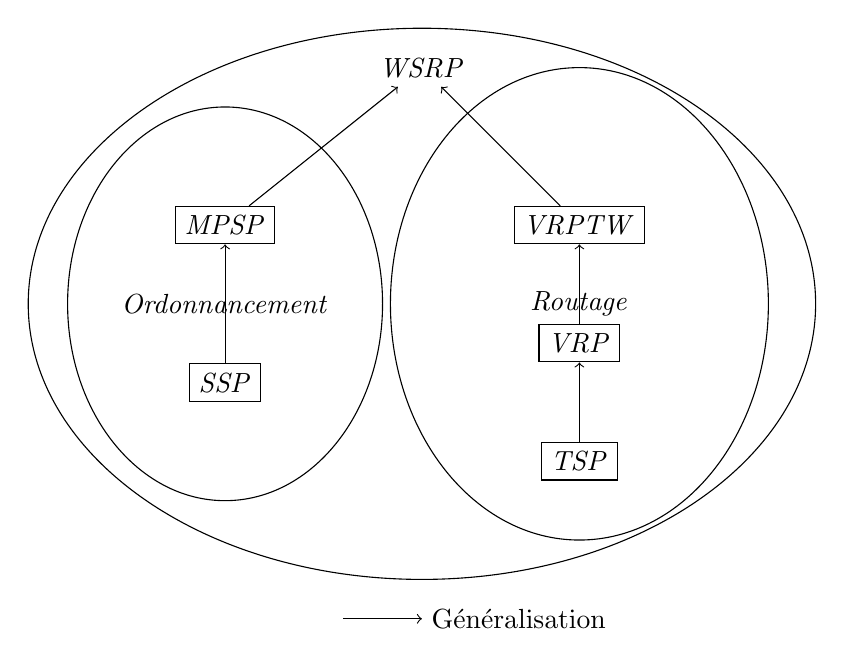
\begin{tikzpicture}
\node[] (0) at (0,0) {\textit{WSRP}};
\draw (0,-3) circle(5 and 3.5);
\draw (2,-3) circle(2.4 and 3) node[]{\textit{Routage}};
\draw (-2.5,-3) circle(2 and 2.5) node[]{\textit{Ordonnancement}};
\node[draw,rectangle] (4) at (-2.5,-4) {\textit{SSP}};

\node[draw,rectangle] (5) at (2,-3.5) {\textit{VRP}};
\node[draw,rectangle] (9) at (2,-5) {\textit{TSP}};

\draw[->] (9)--(5);

\node[draw,rectangle] (1) at (-2.5,-2) {\textit{MPSP}};
\node[draw,rectangle] (2) at (2,-2) {\textit{VRPTW}};
\draw[->] (4)--(1);
\draw[->] (5)--(2);

\draw[->] (2)--(0);
\draw[->] (1)--(0);
\draw[->] (-1,-7)--(0,-7) node[right] {Généralisation};
\end{tikzpicture}
\caption{Schéma représentant la classe de complexité de la classe WSRP \label{fig:complex:gloabale}}
\end{figure}


La figure~\ref{fig:complex:gloabale} représente les généralisations successives des problèmes d'ordonnancement et de routage de base, comme le \tsp, qui mènent à la classe de problèmes \wsrp.
Lorsque l'on dit qu'un problème $\pi_1$ est une généralisation d'un autre $\pi_2$ (ou alors que $\pi_2$ généralise $\pi_1$) cela veut dire qu'il est plus dur au sens de la complexité. 
Si on passe des instances de $\pi_2$ à $\pi_1$ alors ces instances n'utilisent qu'un sous-ensemble des contraintes de $\pi_1$.
Autrement dit, on peut modéliser des instances plus complexes en utilisant $\pi_1$ qu'en utilisant $\pi_2$.


\begin{comment}

\begin{figure}[H]

\centering
\begin{tikzpicture}

\node[draw,rectangle] (0) at (0,0) {\wsrp};

\node[draw,rectangle] (1) at (-2,-2) {\mpsp};
\node[draw,rectangle] (2) at (0,-2) {\vrptw};
\node[draw,rectangle] (3) at (2.5,-2) {\pdptw};

\node[draw,rectangle] (4) at (-2,-4) {\ssp};
\node[draw,rectangle] (5) at (0,-4) {\vrp};
\node[draw,rectangle] (6) at (2.5,-3) {\pdp};

\node[draw,rectangle] (7) at (-2.7,-6) {\rcpsp};
\node[draw,rectangle] (8) at (-1.2,-6) {$\ldots$};
\node[draw,rectangle] (9) at (0,-6) {\tsp};

\draw[->] (1)--(0);
\draw[->] (2)--(0);
\draw[->] (3)--(0);

\draw[->] (4)--(1);
\draw[->] (5)--(6);
\draw[->] (5)--(2);
\draw[->] (6)--(3);

\draw[->] (7)--(4);
\draw[->] (8)--(4);
\draw[->] (9)--(5);
%%%%%%%%%%%%% Légendes %%%%%%%%%%%%%%
\draw[->] (3.5,-5)--(4,-5);
\node[] at (3,-5) {A};
\node[] at (4.5,-5) {B};
\node[] at (3.75,-5.5) {$=$};
\node[] at (3.75,-6) {B généralise A};
\end{tikzpicture}

\caption{\label{Fig:Complexite} \'Evolution des problèmes : ajout de contraintes }
\end{figure}
\end{comment}

En ce qui concerne les méthodes de résolution, Rasmussen et al. \cite{Rasmussen2010} proposent une formulation MIP, et utilisent la génération de colonnes et une décomposition de Dantzig-Wolfe avec différentes méthodes de branchements dans l'algorithme de branch-and-price. Cependant avec leur méthode, ils ne résolvent pas à l'optimal des instances avec 15 employés, 150 tâches et environs 30\% de tâches avec des contraintes de précédences en moins de 20 minutes.

Xie et al. \cite{Xie2017} utilisent de la recherche locale itérée (iterated local search) pour résoudre des instances d'un problème de \wsrp.
Leur méthode est la suivante : ils construisent une solution réalisable, puis avec des opérateurs de voisinage (échange ou inversion de séquence) puis améliorent la solution jusqu'à potentiellement obtenir la solution optimale, cependant on perd la garantie d'optimalité et même de qualité de solution : on ne connaît pas l'écart entre la solution trouvée et la solution optimale.
Ils comparent leur méthode de résolution à une résolution exacte et à de l'ALNS sur des instances avec 30 techniciens et 100 tâches.
L'avantage de leur méthode est que la solution obtenue est de bonne qualité (gap de 1\%) et le vrai avantage est le temps d'exécution (moins d'une minute) alors que la recherche exacte (modèle MIP + cplex) utilisée met au plus 2 heures pour trouver la solution optimale.


%%%%%%%%%%%%%%%%%%%%%%%%%%%%%%%%%%%%%%%
%%%%%%%%%%%%%%%%%%%%%%%%%%%%%%%%%%%%%%%

%\section{Complexité \label{sec:SOA_Complex}}
%
\begin{mydef}
La classe $\p$ contient tous les problèmes de décision pour lesquelles on peut trouver une réponse avec une machine de Turing en un nombre d'étapes borné par une fonction polynomiale en la taille des entrées.
\end{mydef}
\begin{mydef}
La classe $\np$ contient tous les problèmes de décision pour lesquelles on peut vérifier une solution correcte avec une machine de Turing en un nombre d'étapes borné par une fonction polynomiale en la taille des entrées.
\end{mydef}
\begin{mydef}
Un problème $\pi$, de décision ou d'optimisation, est $ \np-difficile$ si tous les problèmes de la classe $\np$ admettent une réduction polynomiale vers $\pi$. 
\end{mydef}


\wsrp combine la complexité des problèmes d'ordonnancement \cite{Blazewicz1983,Lageweg1982} : ordonnancement de projet à compétences multiples (Multi-skill Project Scheduling Problem, Tehcnician and Task Scheduling Problem), séquençage et ordonnancement de tâches (Sequencing and Scheduling Problem) \cite{Lawler1993}, ordonnancement de projet avec contraintes de ressources (Resources Constrained Project Scheduling Problem) et des problèmes de tournée de véhicule \cite{Lenstra2013,Tsitsiklis1992} : problème de tournée de véhicule avec fenêtre de temps (Vehicule Routing Problem with Time Windows), problème de tournée de véhicule avec fenêtre de temps, dépendance temporelle (Vehicle Routing Problem with Time Windows and Time Dependancies) et Traveling Salesman Problem with Time Windows. Nous allons avoir besoin de définir quelques problèmes  avant de pouvoir définir la complexité de \wsrp.









%\probdef{Un graphe $G=(V,E,\omega)$ non orienté et M < |V|.}{Trouver $m\leq M$ cycles disjoints de coût Min couvrant V}{Vehicule Routing Problem}{VRP}{def:VRP}


\indent 


\begin{comment}
La Figure~\ref{Fig:Complexite} montre le lien entre les problèmes défini plus haut.


\begin{figure}[H]
\centering
\includegraphics[scale=0.4]{RCPSP}
\caption{\label{RCPSP} Exemple de problème d'ordonnancement de projet avec contrainte de ressources.La ligne en pointillé représente la contrainte de ressources, l'ordonnancement du bas est une solution réalisable alors que celui du haut est une solution qui ne respecte pas la contrainte de ressource}
\end{figure}
\end{comment}

\begin{comment}



\begin{defPb}{Le problème d'ordonnancement de techniciens et de tâches}{Technician and Task Scheduling Problem}

\end{defPb}



\begin{defPb}{Le problème d'ordonnancement et de routage de techniciens}{Technician Routing and Scheduling Problem} \cite{zamorano2017branch} est majoritairement présent dans le domaine de la maintenance d'équipement et d'installation dans des bâtiments.
\end{defPb}

\begin{defPb}{Le problème d'Assistance à Domicile} {Home Care Problem} vise à assisté des personnes âgées ou handicapée pour effectuer des tâches quotidiennes (faire les courses, se préparer à manger, etc). \cite{akjiratikarl2007pso}
\end{defPb}

\begin{defPb}{Le problème de planning d'infirmière} {Nurse Scheduling/Nurse Rostering Problem} est un problème qui possède beaucoup de contraintes souvent séparé en contraintes "molles" (soft constraint) qui peuvent être violées mais cela à un coût et contraintes "dures" (hard constraint) qui ne peuvent pas être violées \cite{Trilling2007}. L.  
\end{defPb}



\begin{defPb}{Le problème de Soins Infirmiers à Domicile}{Home Health Care Problem} est une extension du problème de planning d'infirmière. En effet en plus de fournir un planning qui respecte les préférences des infirmières, il faut associé à chaque infirmière une tournée qui minimise le temps de trajet entre chaque visite. On peut le voir aussi comme une variante de \trsp \cite{Bertels2006,Rasmussen2010}.
\end{defPb}

\begin{defPb}{Le problème de Planning et Routage de Personnel de Sécurité}{Security Personal Routing and Rostering} est un problème possède à la fois la dimension de routage (Multi Depot Vehicule Routing Problem) et la dimension d'ordonnancement (Multi-skill Project Scheduling Problem) et pour chacune de ces dimensions le problème est assez contraint. Le problème est assez similaire au problème de Soins Infirmiers à Domicile mais l'horizon du planning est beaucoup plus long \cite{misir2011security}.
\end{defPb}

\begin{defPb}{Le problème de Répartition de Main-d’œuvre}{Manpower Allocation}\cite{lim2004}
\end{defPb}

\begin{defPb}{Le problème de ramassage/récolte et livraison}{Pick-up and Delivery Problem} \cite{Ropke2005}
\end{defPb}

\begin{figure}[H]
\centering
\includegraphics[scale=0.8]{PDP}
\caption{Exemple de routage pour le \pdp\label{fig:PDP}}
\end{figure}
\end{comment}

%%%%%%%%%%%%%%%%%%%%%%%%%%%%%%%%%%%%%%%
%%%%%%%%%%%%%%%%%%%%%%%%%%%%%%%%%%%%%%%



%%%%%%%%%%%%%%%%%%%%%%%%%%%%%%%%%%%%%%%
%%%%%%%%%%%%%%%%%%%%%%%%%%%%%%%%%%%%%%%

%\section{Techniques actuelles d'optimisation\label{sec:SOA_Optim}}
%Dans cette section nous allons discuter des techniques d'optimisation pour résoudre le problème. Comme pour tous les problèmes d'optimisation plusieurs méthodes de résolution s'opposent : les méthodes exactes, les méthodes approchées avec garanties de performances, les méthodes \mbox{(méta-)heuristiques} ou alors des méthodes hybrides qui mélangent les méthodes de résolutions ci-dessus. Le choix des méthodes de résolution est fortement lié aux critères de résolution du problème, par exemple si l'on peut se permettre de résoudre le problème dans un temps raisonnable on va favoriser les méthodes exactes. Les méthodes approchées visent à obtenir une "bonne" solution rapidement.
\begin{mydef}
\label{def:exact2}
Une méthode exacte parcourt l'arbre de recherche du problème afin de trouver la meilleure solution avec une garantie d'optimalité.
\end{mydef}
\begin{mydef}
\label{def:greedy2}
Un algorithme glouton (greedy algorithm) est un algorithme qui étape après étape améliore la solution actuelle jusqu'à un extremum local (parfois global). 
\end{mydef}
\begin{mydef}
\label{def:metaheuristic2}
Une méta-heuristique est une méthode permettant de trouver un extremum local pour un problème d'optimisation. Le fonctionnement général d'une méta-heuristique est de parcourir un "voisinage" d'une solution courante en cherchant a optimiser une fonction objectif. Il existe un grand nombre de méta-heuristiques allant de la simple recherche locale vers des algorithmes génétiques au comportements plus complexes.
\end{mydef}

Rasmussen et al. \cite{Rasmussen2010} proposent une formulation MIP, et utilisent une décomposition de Dantzig-Wolfe avec différentes méthodes de branchements dans l'algorithme de de branch-and-price. Cependant avec leur méthode, ils ne résolvent pas à l'optimal des instances avec 15 employés, 150 tâches et environs 30\% de tâches avec des contraintes de précédences en moins de 20 minutes.

Xie et al. \cite{Xie2017} utilisent de la recherche locale itérée (iterated local search) pour résoudre des instances d'un problème de \wsrp. Leur méthode est la suivante : ils construisent une solution réalisable, puis avec des opérateurs de voisinage (échange ou inversion de séquence) ils améliorent la solution jusqu'à potentiellement . Ils comparent leur méthode de résolution à une résolution exacte et à de l'ALNS sur des instances avec 30 techniciens et 100 tâches. L'avantage de leur méthode est que la solution obtenu est de bonne qualité (gap de 1\%) et le vrai avantage est le temps d'exécution (moins d'une minute) alors que la recherche exacte (modèle MIP + cplex) utilisent met au plus 2h pour trouver la solution optimale.

Dans la littérature toutes ces méthodes de résolution s'affrontent. 
methodes exactes MIP contrainte dantzig-Wolfe decomp, branching method lower bound\\
meta-heuristiques tabu, recuit simulé, génétique PSO, ALNS, pALNS, \\
heuristiques Iterated local search, LNS,\\
glouton, assignement problem,\\
multi obj\\
relaxation lineaire CP + MIP\\

%%%%%%%%%%%%%%%%%%%%%%%%%%%%%%%%%%%%%%%
%%%%%%%%%%%%%%%%%%%%%%%%%%%%%%%%%%%%%%%

\section{Limites de l'état de l'art\label{sec:SOA_Limites}}
La plupart des problèmes en recherche opérationnelle sont $\mathcal{NP}$-difficiles au sens fort. Par exemple trouver une solution réalisable pour le problème de tournée de véhicules avec contraintes de fenêtres temporelles a été montré $\mathcal{NP}$-complet \cite{Desrosiers1995}.
En pratique il est difficile de trouver une solution en un temps raisonnable pour des problèmes de recherche opérationnelle pour des instances de grande taille.

En général la réalité opérationnelle fait face aux résultats théoriques. D'une part les résultats théoriques apportent des méthodes de résolution efficaces (qui donnent une solution proche de l'optimal avec un faible temps de résolution).
Cependant lorsque l'on passe aux instances industrielles ces méthodes de résolution ne sont plus aussi efficaces, à cause du volume des données mais aussi à cause de la limitation du temps de résolution.
Dans le monde opérationnel il faut aller vite pour résoudre de grandes instances. Ce qui a pour conséquence de s'écarter de la garantie d'optimalité ou d'approximation (utilisation de méta-heuristiques).


Le volume des données est un facteur important dans la résolution d'un problème, surtout pour les problèmes $\np$-difficile au sens fort car le temps de résolution croit exponentiellement avec l'augmentation de la taille de l'instance.

Nous devons résoudre tous les jours des instances de notre problème avec 150-200 techniciens et environs 10 000 tâches en moins d'une heure. 
Les instances résolues dans la littérature en moins d'une heure sont bien plus petites que celles que nous devons résoudre, cependant elles sont souvent résolues à l'optimal.
En conséquence les temps de résolution sont trop longs, nous devons résoudre chaque instance en moins d'une heure. 
Il faudra donc prendre en compte la différence de taille des instances pour les méthodes de résolution que nous utiliserons. 
A priori nous ne pourrons pas résoudre nos instances à l'optimal ou alors nous n'aurons pas de garantie sur l'optimalité de la solution obtenue.


%%%%%%%%%%%%%%%%%%%%%%%%%%%%%%%%%%%%%%%
%%%%%%%%%%%%%%%%%%%%%%%%%%%%%%%%%%%%%%%

